\chapter{Proposed System and Design}

\section{Proposed System}

The proposed system is a smartphone-based platform that combines computer vision, GPS telemetry, and weather intelligence to give drivers reliable and context-aware safety assistance. The system is divided into five modules.

\begin{enumerate}
    \item \textbf{Vision and Object Detection Module:} Captures real-time road scenes using the smartphone camera and detects vehicles and obstacles using a lightweight YOLOv8 Nano model.
    \item \textbf{Telemetry and GPS Module:} Collects real-time speed, location, and bearing data from the smartphone's built-in GPS receiver to track driving behavior.
    \item \textbf{Environmental Context Module:} Retrieves live weather and visibility conditions via external APIs based on the current location.
    \item \textbf{Risk Engine and Reasoning Module:} Combines visual, telemetry, and environmental data to calculate a continuous driving risk score and provides transparent explanations for its assessment.
    \item \textbf{User Interface Module:} Displays the live camera feed, current risk status, warnings, and safety recommendations through an intuitive dashboard.
\end{enumerate}

The working of the system in brief is as follows. The driver mounts the smartphone on the dashboard and starts the application. The camera begins capturing the road ahead, while the GPS receiver continuously tracks vehicle speed and location. The environmental module simultaneously checks the local weather conditions. The risk engine processes these inputs together---evaluating the distance to detected vehicles, current speed, and weather-related visibility---to determine a driving risk score. If a hazard or unsafe condition is detected, the reasoning module generates a transparent explanation. Finally, the user interface displays the live feed alongside context-aware visual warnings and safety recommendations to assist the driver.

\section{Feasibility Study}

\subsection{Technical Feasibility}
The system uses computer vision algorithms, smartphone sensors, weather APIs, and mobile application technologies, all of which are mature and well documented. It can be developed using open source frameworks like Flutter and Google LiteRT, alongside lightweight object detection models such as YOLOv8 Nano. Since modern smartphones are equipped with high-quality cameras and GPS receivers, the integration of on-device processing without external computing hardware is technically possible. Existing research has already shown that monocular camera-based perception and telematics-based risk assessment work in practice for driver assistance.

\subsection{Operational Feasibility}
The system provides a simple and intuitive dashboard interface for drivers with different technical backgrounds. It delivers real-time risk assessment, visual warnings, and transparent safety recommendations to improve driving decisions. Since the application runs entirely on the driver's smartphone mounted on the dashboard, it requires minimal setup and integrates easily into daily driving routines. The clear, explicit reasoning provided alongside alerts ensures that the system is easily understandable and builds user trust without causing cognitive overload.

\subsection{Economic Feasibility}
The project reduces the likelihood of accidents through proactive risk assessment and timely safety warnings. The development cost is low because open source software frameworks and freely available AI models are used. Unlike traditional Advanced Driver Assistance Systems (ADAS) that require expensive, specialized vehicle hardware, this system leverages the smartphone the user already owns. The minimal cost associated with standard mobile data usage for weather APIs makes the system highly affordable. The expected improvement in driver safety and accident prevention is significantly greater than the minimal operational cost of the system.

\section{Design}
The design of the system is user centric and modular. The main design diagrams are explained below.

\subsection{Architecture Diagram}
An architecture diagram provides an overall view of the major components of a software system and the connections between them. The architecture of the ContextDrive system consists of five main layers, as shown in Figure~\ref{fig:arch}.

\begin{figure}[H]
    \centering
    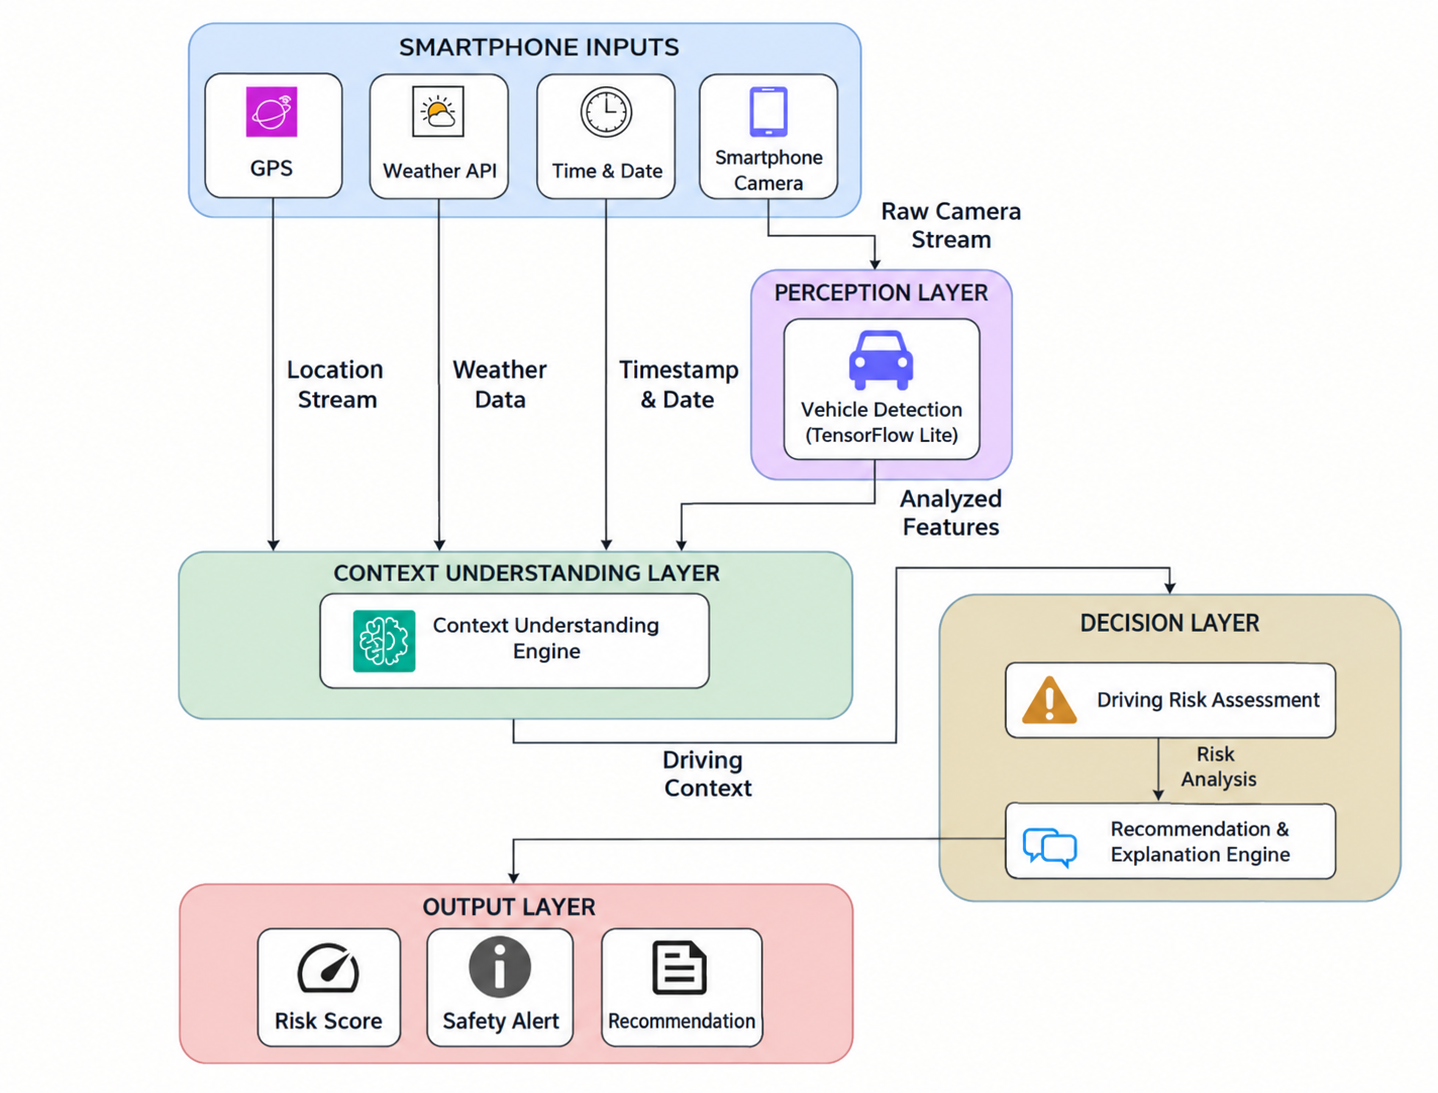
\includegraphics[width=\textwidth]{img/arch_diagram.png}
    \caption{Architecture Diagram of ContextDrive}
    \label{fig:arch}
\end{figure}

\begin{enumerate}
    \item \textbf{Input Layer:} This layer is the primary source of raw data for the system, originating from a user's smartphone. It groups several distinct data sources:
    \begin{itemize}
        \item \textit{GPS:} Outputs a location stream to the context understanding layer.
        \item \textit{Weather API:} Outputs weather data based on the current location.
        \item \textit{Time \& Date:} Outputs timestamp and date information.
        \item \textit{Smartphone Camera:} Outputs a raw camera stream to the perception layer.
    \end{itemize}
    \item \textbf{Perception Layer:} This layer processes raw sensor data from the input layer to detect environmental features. The vehicle detection engine analyzes visual data, receiving the raw camera stream and outputting analyzed features regarding detected vehicles and objects.
    \item \textbf{Context Understanding Layer:} This central layer consolidates diverse data points to create a comprehensive understanding of the current driving environment and situation. The context understanding engine builds a high-level situational model by receiving the location stream, weather data, timestamp, and analyzed features, ultimately generating a critical data stream called the driving context.
    \item \textbf{Decision Layer:} This layer analyzes the comprehensive driving context to assess risk and formulate advice in two connected stages:
    \begin{itemize}
        \item \textit{Driving Risk Assessment:} Evaluates the context data for potential hazards and risk levels, generating a risk analysis stream.
        \item \textit{Recommendation \& Explanation Engine:} Generates actionable advice and the rationale behind that advice based on the risk analysis, resulting in a consolidated assessment and recommendation stream.
    \end{itemize}
    \item \textbf{Output Layer:} This final layer presents the system’s findings and advice to the user. It receives the high-level driving context and the assessment and recommendation data. The presentation modules include the Risk Level, Safety Alert, and Recommendation.
\end{enumerate}

\subsection{Use Case Diagram}
The use case diagram illustrates the main functionalities of the ContextDrive system and the interactions of its primary actor, the driver. The driver can start a trip, view the live camera dashboard, and receive real-time driving risk assessments based on speed and proximity. The driver can also review the transparent safety explanations generated by the system to understand the factors influencing the current warnings.

\begin{figure}[H]
    \centering
    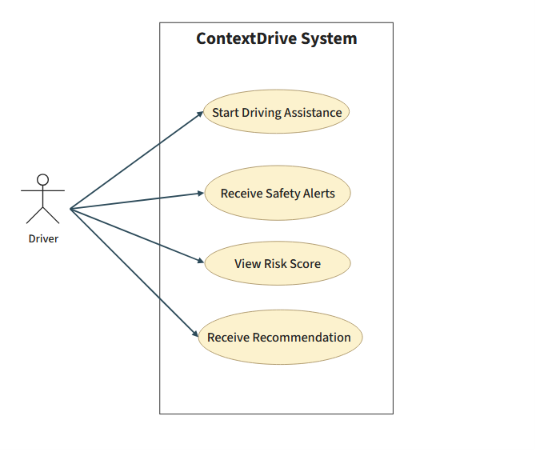
\includegraphics[width=0.8\textwidth]{img/use_case_diagram.png}
    \caption{Use Case Diagram}
    \label{fig:use_case}
\end{figure}

\subsection{Level 0 DFD}
Level 0 represents the complete ContextDrive system as a single process, as shown in Figure~\ref{fig:dfd0}. It illustrates the high-level flow of information:
\begin{itemize}
    \item \textbf{Driving Context Data (Input):} Raw environmental and sensor data (location, weather, time, camera) fed into the system.
    \item \textbf{ContextDrive (Processing):} The core engine that receives the raw data, analyzes the driving situation, and evaluates potential risks.
    \item \textbf{Risk Alerts \& Driving Recommendations (Output):} The final result generated by ContextDrive, delivering safety warnings and driving advice to the user.
\end{itemize}

\begin{figure}[H]
    \centering
    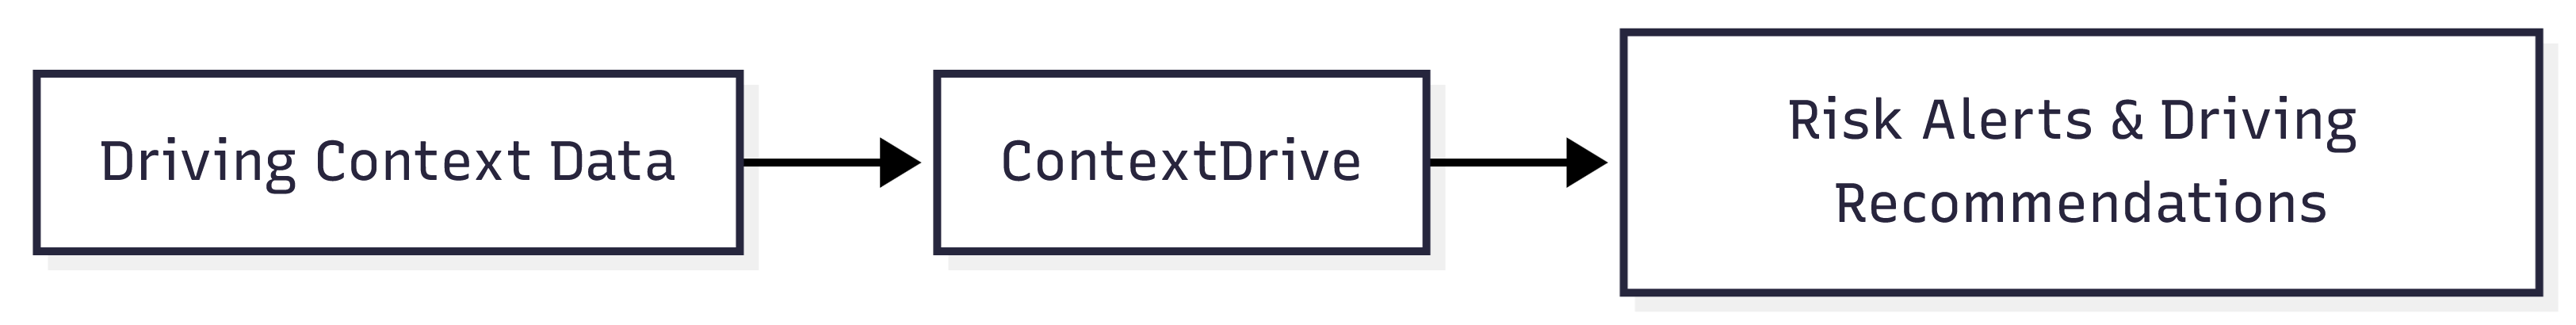
\includegraphics[width=0.9\textwidth]{img/dfd_0.png}
    \caption{Data Flow Diagram - Level 0}
    \label{fig:dfd0}
\end{figure}

\subsection{Level 1 DFD}
Level 1 decomposes the ContextDrive system into major processes, as shown in Figure~\ref{fig:dfd1}. The flow is structured as follows:
\begin{itemize}
    \item \textbf{Inputs:} Four external data sources feed into the central system:
    \begin{itemize}
        \item \textit{Smartphone Camera:} Sends Camera Frames.
        \item \textit{Smartphone GPS:} Sends Speed / Location.
        \item \textit{Weather API:} Sends Weather Data.
        \item \textit{Smartphone Clock:} Sends Time \& Date.
    \end{itemize}
    \item \textbf{ContextDrive System:} The central processing hub that receives and combines all four input streams.
    \item \textbf{Driver:} The final recipient who receives the Risk Score, Safety Alerts, and Recommendations generated by the ContextDrive System.
\end{itemize}

\begin{figure}[H]
    \centering
    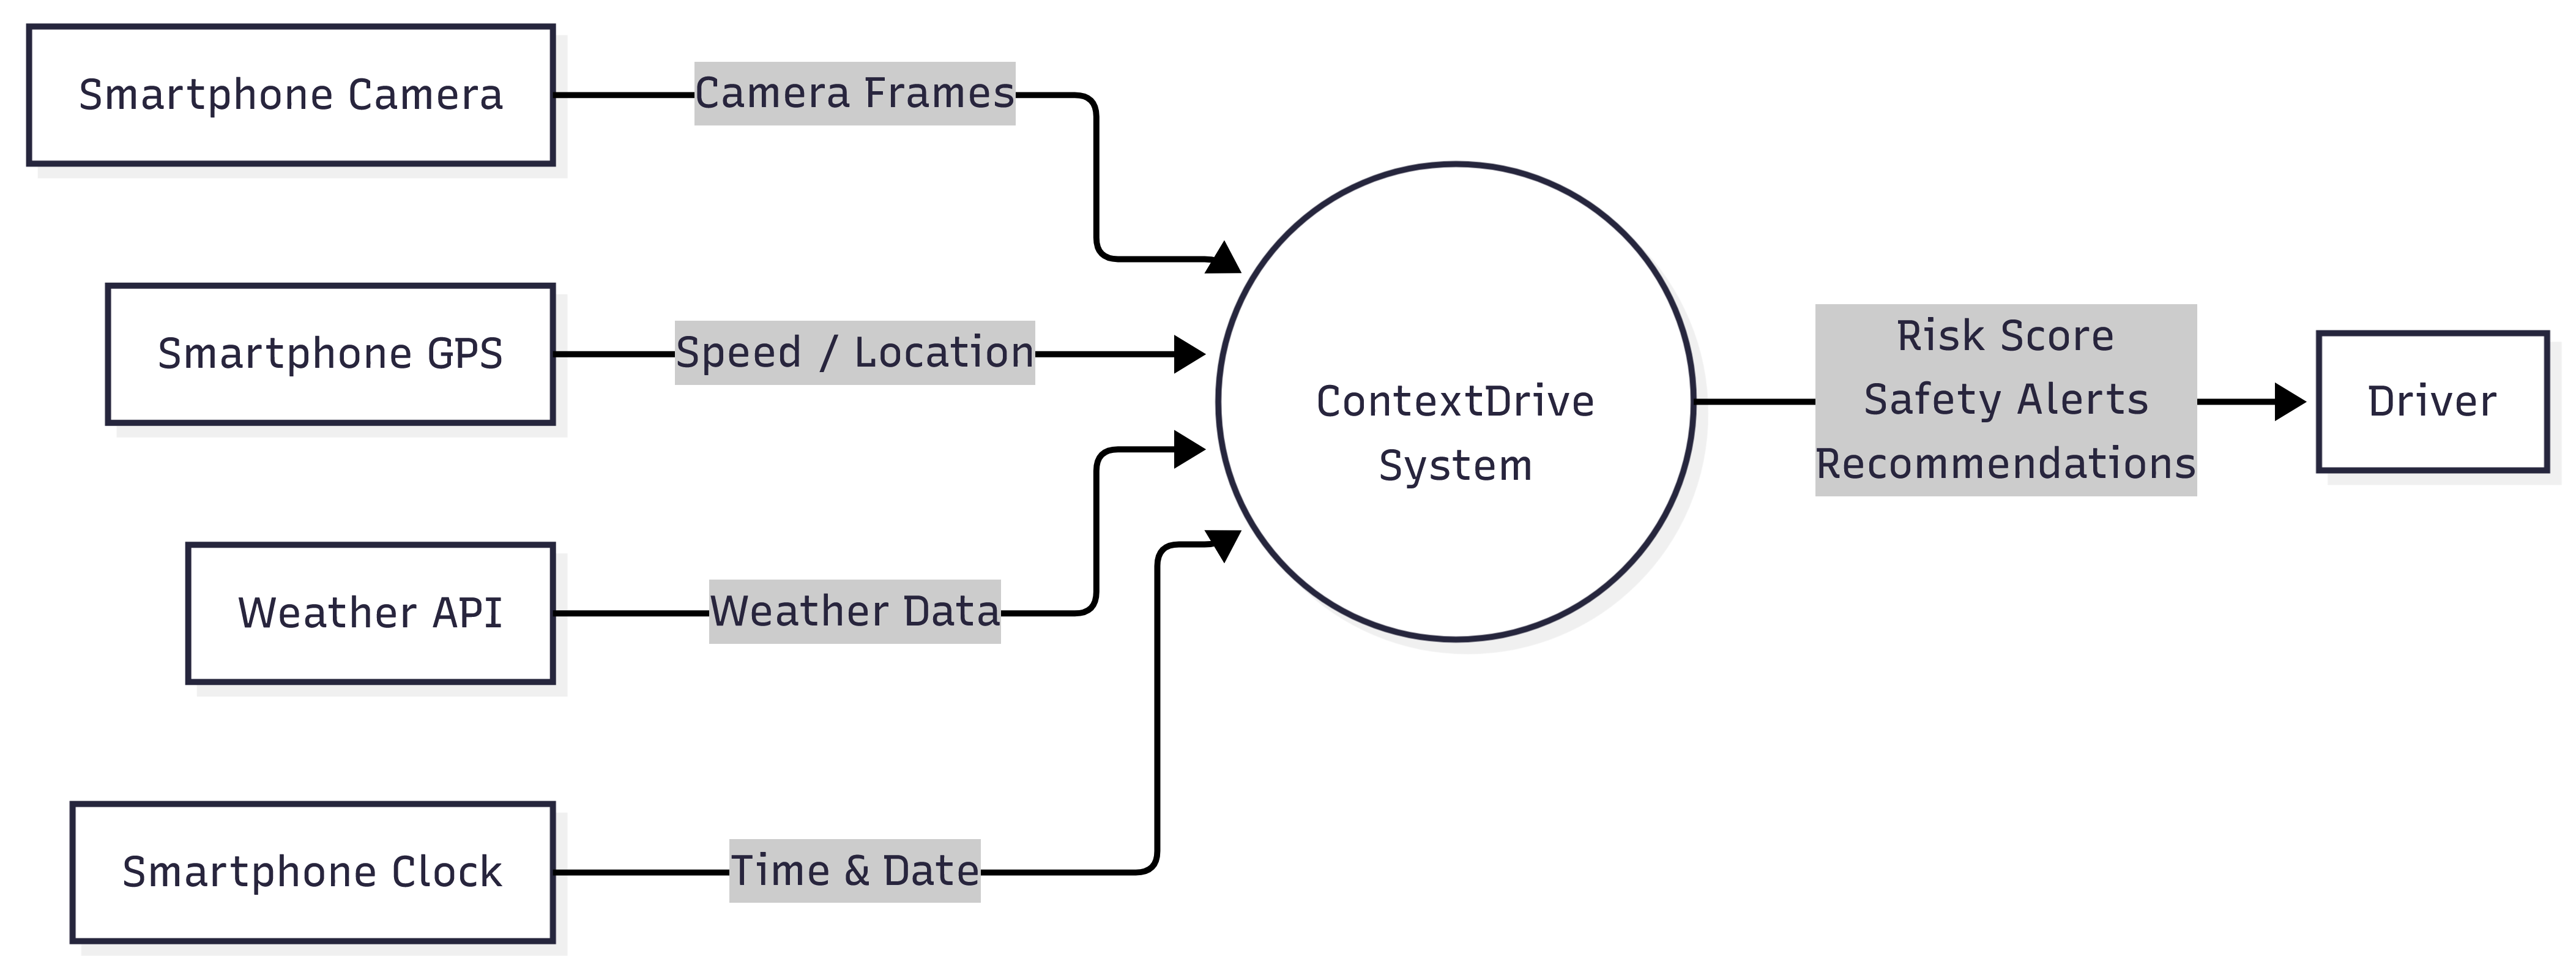
\includegraphics[width=0.9\textwidth]{img/dfd_1.png}
    \caption{Data Flow Diagram - Level 1}
    \label{fig:dfd1}
\end{figure}

\subsection{Level 2 DFD}
Level 2 DFD provides a more detailed view of the internal sub-processes within the core modules of the system, as shown in Figure~\ref{fig:dfd2}.
\begin{itemize}
    \item \textbf{Inputs:}
    \begin{itemize}
        \item \textit{Smartphone Camera:} Sends Camera Frames to the Vehicle Detection process.
        \item \textit{Smartphone GPS:} Sends Speed/Location to the Context Understanding process.
        \item \textit{Weather API:} Sends Weather Data to the Context Understanding process.
        \item \textit{Smartphone Clock:} Sends Time \& Date to the Context Understanding process.
    \end{itemize}
    \item \textbf{Processes:}
    \begin{itemize}
        \item \textit{Vehicle Detection:} Receives Camera Frames and outputs Vehicle Information to the Context Understanding process.
        \item \textit{Context Understanding:} Combines Vehicle Information, Speed/Location, Weather Data, and Time \& Date to output Driving Context to the Driving Risk Assessment process.
        \item \textit{Driving Risk Assessment:} Analyzes the Driving Context and sends a Risk Score to the Recommendation \& Explanation process.
        \item \textit{Recommendation \& Explanation:} Takes the Risk Score and sends the final Alert and Recommendation to the Driver.
    \end{itemize}
    \item \textbf{Output:}
    \begin{itemize}
        \item \textit{Driver:} The final recipient who receives the Alert and Recommendation from the Recommendation \& Explanation process.
    \end{itemize}
\end{itemize}

\begin{figure}[H]
    \centering
    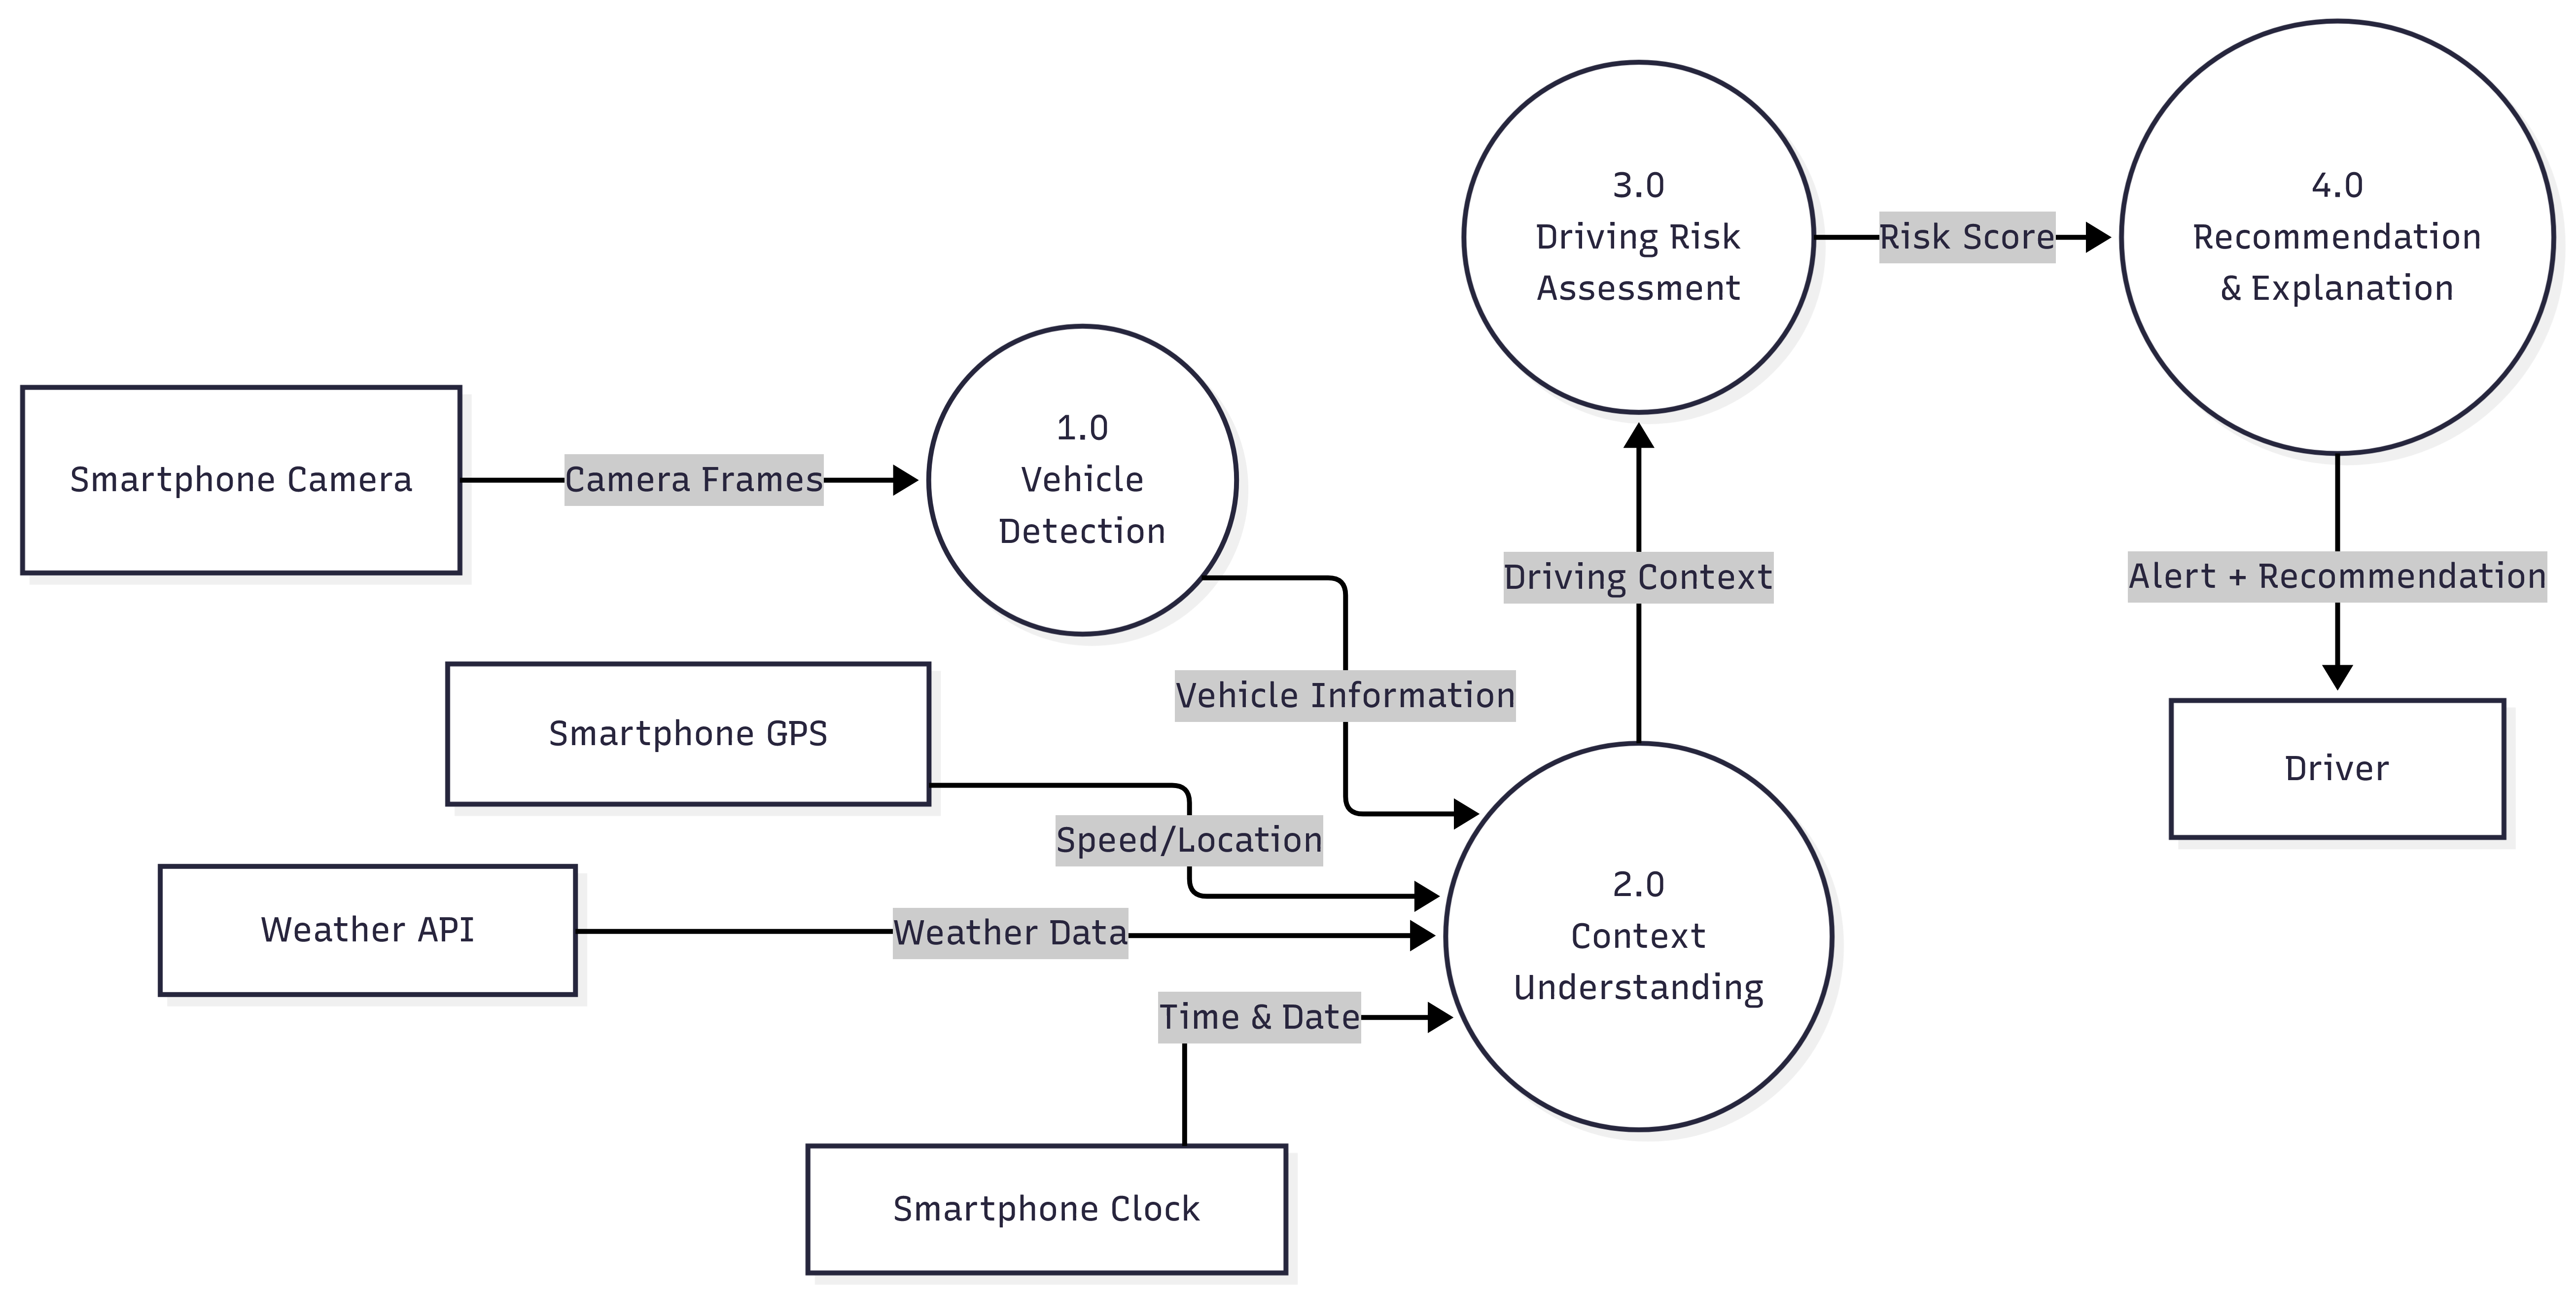
\includegraphics[width=0.9\textwidth]{img/dfd_2.png}
    \caption{Data Flow Diagram - Level 2}
    \label{fig:dfd2}
\end{figure}

\subsection{Methods and Techniques}
The ContextDrive system integrates various methods and techniques to support drivers in making informed, safe decisions. The system combines computer vision-based object detection, GPS telemetry tracking, weather data analysis, deterministic risk assessment, and transparent explainability mechanisms. These techniques work together to provide personalized and data-driven safety recommendations.

\noindent\textbf{Computer Vision-Based Object Detection}\\
The system uses the YOLOv8 Nano model via Google LiteRT to detect vehicles and obstacles in the live camera feed. This lightweight model processes camera frames efficiently on-device, providing bounding boxes and proximity estimations for critical road elements.

\vspace{0.5em}
\noindent\textbf{GPS Telemetry Tracking}\\
The system collects real-time speed, location, and bearing data from the smartphone's built-in GPS receiver. This telemetry data is used to continuously monitor the vehicle's dynamic state and movement patterns.

\vspace{0.5em}
\noindent\textbf{Weather Data Analysis}\\
Weather and visibility information is obtained using the OpenWeatherMap API based on current GPS coordinates. Parameters such as visibility distance, precipitation, and extreme weather alerts are incorporated to adjust the risk sensitivity of the system.

\vspace{0.5em}
\noindent\textbf{Deterministic Risk Assessment}\\
The system employs a rule-based deterministic risk engine to calculate a continuous driving risk score. It evaluates multiple factors, including vehicle speed, proximity to detected objects, and adverse weather conditions, to classify the driving situation into distinct risk levels.

\vspace{0.5em}
\noindent\textbf{Transparent Explainability}\\
To build trust and prevent cognitive overload, the system generates clear, explicit explanations alongside its warnings. This ensures the driver understands exactly which environmental or behavioral factors contributed to the current safety alert.

\vspace{0.5em}
\noindent\textbf{Real-Time Driver Interface}\\
The application provides a responsive Flutter-based dashboard that overlays the risk score, safety alerts, and actionable recommendations directly onto the live camera feed, ensuring seamless integration into the driving experience.